% -*- latex -*-
%%%%%%%%%%%%%%%%%%%%%%%%%%%%%%%%%%%%%%%%%%%%%%%%%%%%%%%%%%%%%%%%
%%%%%%%%%%%%%%%%%%%%%%%%%%%%%%%%%%%%%%%%%%%%%%%%%%%%%%%%%%%%%%%%
%%%%
%%%% This text file is part of the source of 
%%%% `Parallel Programming in MPI and OpenMP'
%%%% by Victor Eijkhout, copyright 2012-2023
%%%%
%%%% omptopics_course.tex : case studies in OMP
%%%%
%%%%%%%%%%%%%%%%%%%%%%%%%%%%%%%%%%%%%%%%%%%%%%%%%%%%%%%%%%%%%%%%
%%%%%%%%%%%%%%%%%%%%%%%%%%%%%%%%%%%%%%%%%%%%%%%%%%%%%%%%%%%%%%%%

\documentclass[11pt,headernav]{beamer}

\beamertemplatenavigationsymbolsempty
\usetheme{Madrid}%{Montpellier}
\usecolortheme{seahorse}
\setcounter{tocdepth}{1}

\setbeamertemplate{footline}{\hskip1em Eijkhout: OMP topics\hfill
  \hbox to 0in {\hss \includegraphics[scale=.1]{tacclogonew}}%
  \hbox to 0in {\hss \arabic{page}\hskip 1in}}

\usepackage{comment}
\input slides.inex
\input commonmacs
\input acromacs
\input slidemacs
\input coursemacs
\input snippetmacs

\begin{document}
\parskip=10pt plus 5pt minus 3pt

\title{OpenMP case studies}
\author{Victor Eijkhout}
\date{SDS 335 2022}

\begin{frame}{}
  \titlepage
\end{frame}

\begin{frame}{Case study: molecular dynamics}
\end{frame}

\begin{numberedframe}{Formulation}
A particle has $x,y$ coordinates and a mass~$c$.
For two particles $(x_1,y_1,c_1)$, $(x_2,y_2,c_2)$
the force on particle~1 from particle~2 is:
\[ \overrightarrow F_{12} = \frac{c_1\cdot c_2}{\sqrt{ (x_2-x_1)^2+(y_2-y_1)^2 }} \cdot \overrightarrow r_{12} \]
where $\overrightarrow r_{12}$ is the unit vector pointing from particle 2 to~1.
With $n$ particles, each particle~$i$ feels a force
\[ \overrightarrow F_i = \sum_{j\not=i} \overrightarrow F_{ij}.\]
\end{numberedframe}

\begin{numberedframe}{Building blocks}
Let's start with a couple of building blocks.
\cverbatimsnippet{ompmolaux}
\end{numberedframe}

\begin{numberedframe}{Sequential code in C}
  (Probably wrong, but hey, I'm not a physicist)
  
\begin{lstlisting}
void add_force( struct force *f,struct force g ) {
  f->x += g.x; f->y += g.y; f->f += g.f;
}
void sub_force( struct force *f,struct force g ) {
  f->x -= g.x; f->y -= g.y; f->f += g.f;
}
\end{lstlisting}

For reference, this is the sequential code:
\cverbatimsnippet{ompmolplain}
Here $\overrightarrow F_{ij}$ is only computed for $j>i$, and then
added to both $\overrightarrow F_i$ and~$\overrightarrow F_j$.
\end{numberedframe}

\begin{numberedframe}{In C++}
In C++ we can have a class with an addition operator and such:
%
\cxxverbatimsnippet{ompxmolclass}
\cxxverbatimsnippet{ompxmolplus}

Sequential code:
\cxxverbatimsnippet{ompxmolplain}
\end{numberedframe}

\begin{numberedframe}{Exercise}
  Is the outer loop parallelizable? The inner? Both together?
\end{numberedframe}

\begin{numberedframe}{Solution 1: full interactions}
One solution would be to compute the $\overrightarrow F_{ij}$
interactions for all~$i,j$,
so that there are no conflicting writes.

\cverbatimsnippet{ompmoljpar}
\end{numberedframe}

\begin{numberedframe}{C++ variant: overloaded reduction}
In C++ we use the fact that we can reduce on any class
that has an addition operator:
%
\cxxverbatimsnippet{ompxmoljpar}  
\end{numberedframe}

\begin{numberedframe}{Exercise}
This increases the scalar work by a factor of two,
but surprisingly, on a single thread the run time improves:
we measure a speedup of \n{6.51} over the supposedly `optimal' code.
(Why?)

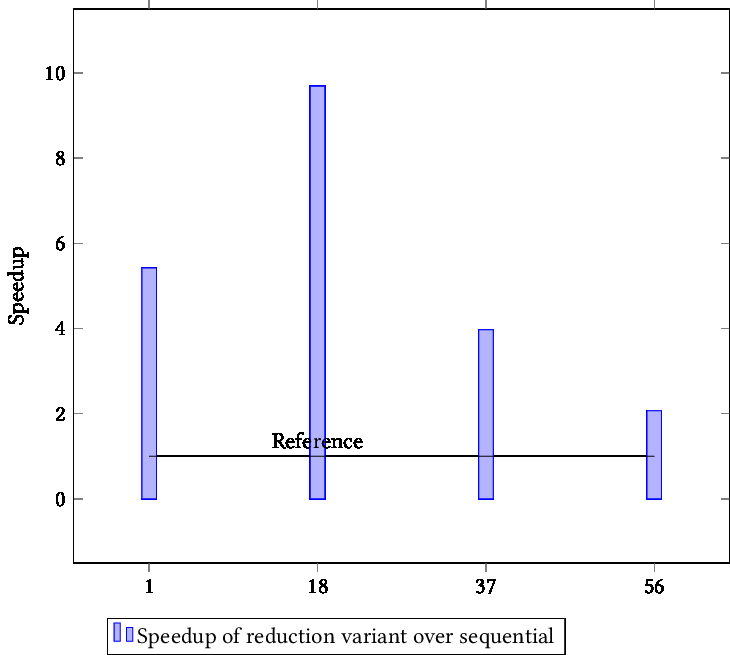
\includegraphics[scale=.6]{omp-nbody1}

What would be an explanation?
\end{numberedframe}

\begin{numberedframe}{Solution 2: atomic updates}
The \n{i} update is fine, we make the \n{j} update atomic:
\cverbatimsnippet{ompmolipar}
To deal with the conflicting \lstinline{jp} writes,
we make the writes atomic:
\begin{lstlisting}
void sub_force( struct force *f,struct force g ) {
#pragma omp atomic
  f->x -= g.x;
#pragma omp atomic
  f->y -= g.y;
#pragma omp atomic
  f->f += g.f;
}
\end{lstlisting}
\end{numberedframe}

\begin{numberedframe}{Result}
  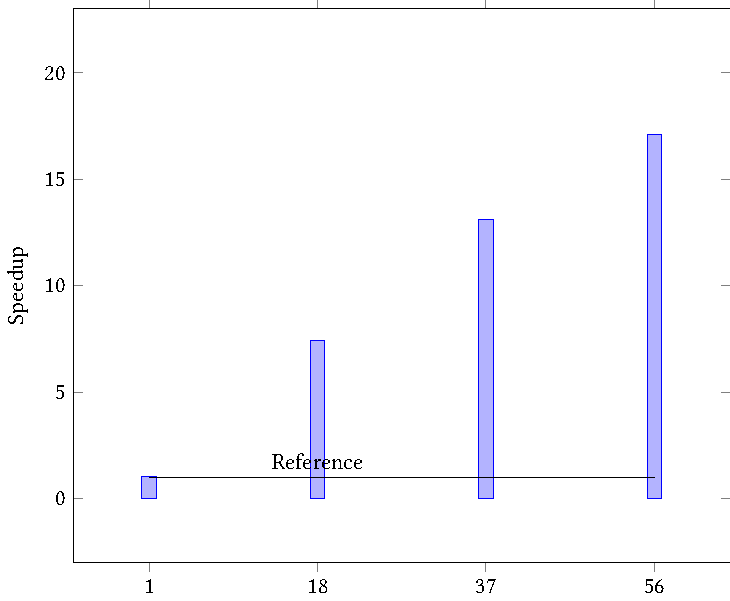
\includegraphics[scale=.6]{omp-nbody2}

  What happens with one thread?
\end{numberedframe}

\begin{numberedframe}{Solution 3: fully atomic}
But if we decide to use atomic updates,
we can take the full square loop,
collapse the two loops,
and make every write atomic.
\cverbatimsnippet{ompmolijpar}
\end{numberedframe}

\begin{numberedframe}{Results}
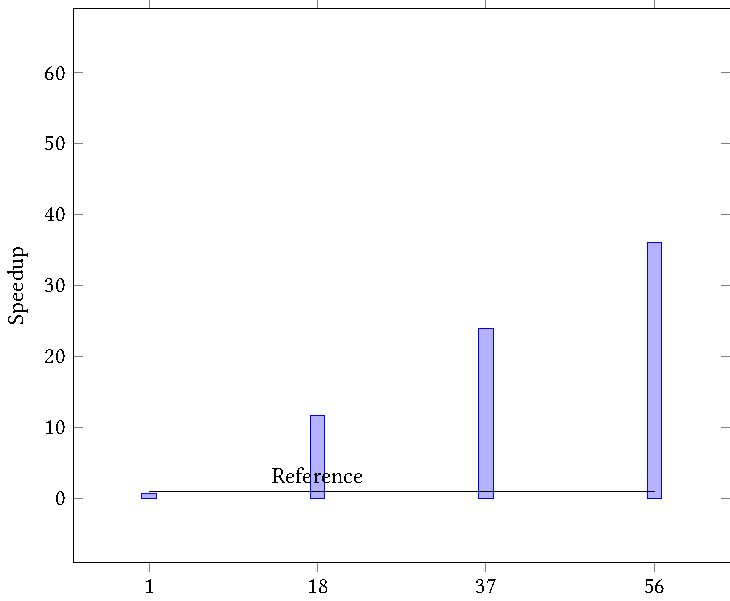
\includegraphics[scale=.6]{omp-nbody3}
\end{numberedframe}

\begin{numberedframe}{All results together}
  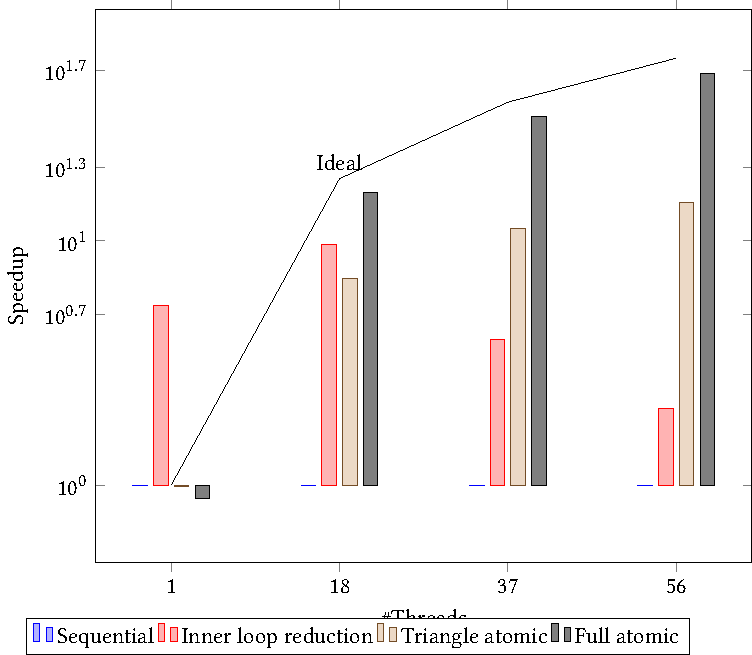
\includegraphics[scale=.6]{omp-nbody4}
\end{numberedframe}

\begin{frame}
  {Search: 8 queens}
\end{frame}

\begin{numberedframe}{Tree traversal}
\begin{multicols}{2}
  Search: traverse the tree, \\
  and abort unsuccessful branches

  DFS, not BFS
  \vfill\hbox{}
  \columnbreak
  \includegraphics[scale=.7]{DFS}
\end{multicols}
\end{numberedframe}

\begin{numberedframe}{Eight queens}
\begin{lstlisting}[language=C++]
placement initial; initial.fill(empty);
auto solution = place_queen(0,initial);

optional<placement> place_queen
        (int iqueen,const placement& current) {
  for (int col=0; col<N; col++) {
    placement next = current;
    next.at(iqueen) = col;
    if (feasible(next)) {
      if (iqueen==N-1)
	return next;
      auto attempt = place_queen(iqueen+1,next);
      if (attempt.has_value())
	return attempt;
    } // end if(feasible)
  }
  return {};
};
\end{lstlisting}
\end{numberedframe}

\begin{numberedframe}{With OpenMP}
\cxxverbatimsnippet{queensmain}
\end{numberedframe}

\begin{numberedframe}{More tasks}
We create a task for each column, and since they are in a loop
we use \indexpragma{taskgroup} rather than \indexpragma{taskwait}.
\begin{lstlisting}[language=C++]
#pragma omp taskgroup
  for (int col=0; col<N; col++) {
    placement next = current;
    next.at(iqueen) = col;
#pragma omp task firstprivate(next)
    if (feasible(next)) {
    // stuff
    } // end if(feasible)
  }
\end{lstlisting}
\end{numberedframe}

\begin{numberedframe}{How to break}
However, the sequential program had \lstinline{return} and \lstinline{break}
statements in the loop, which is not allowed in workshare constructs
such as \indexpragma{taskgroup}.
Therefore we introduce a return variable, declared as shared:
%
\cxxverbatimsnippet{queensbreadth}
\end{numberedframe}

\begin{numberedframe}{Timing}
  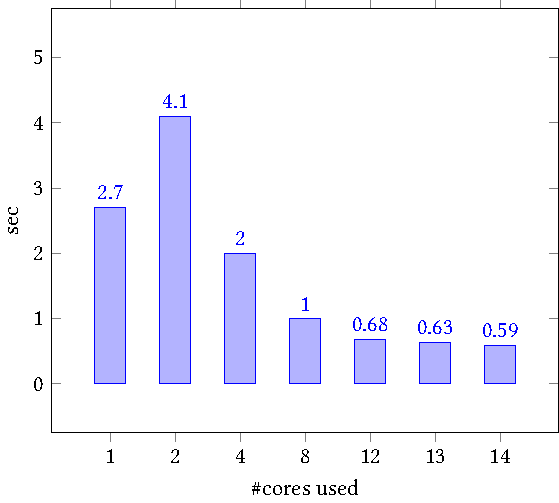
\includegraphics[scale=.6]{omp-dfs-intel}

  This is a 1000 times slower than sequential. Why?
\end{numberedframe}

\begin{numberedframe}{Cancelling}
  Body of the loop over columns:
  
  \cxxverbatimsnippet{queenscancel}
\end{numberedframe}

\begin{numberedframe}{Timing}
  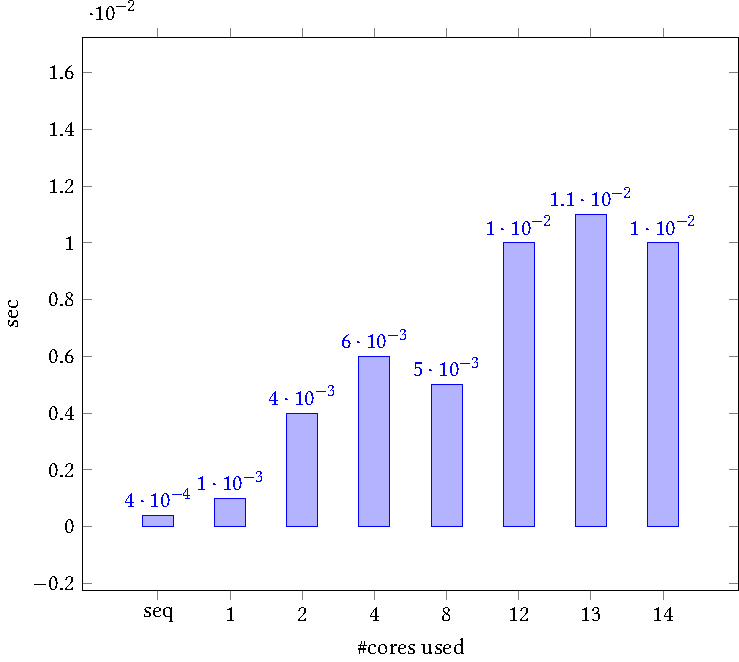
\includegraphics[scale=.6]{omp-dfs-cancel}

  Still not great. Conclusion?
\end{numberedframe}

\begin{frame}
  {C++ notes}
\end{frame}

\begin{numberedframe}{Range syntax}
  Parallel loops in C++ can use range-based syntax:
  %
  \cxxverbatimsnippet{ompcxxloop}
  %
  Tests not reported here show exactly the same speedup as the C~code.
\end{numberedframe}

\begin{numberedframe}{Iterators}
  Support for
  \emph{C++ iterators}\index{C++ iterators!in OMP reduction}
\begin{lstlisting}[language=C++]
#pragma omp declare reduction (merge : std::vector<int>
    : omp_out.insert(omp_out.end(), omp_in.begin(), omp_in.end())) 
\end{lstlisting}
\end{numberedframe}

\begin{numberedframe}{Templated reductions}
  You can reduce with a templated function
  if you put both the declaration and the reduction
  in the same templated function:
  %
  \cxxverbatimsnippet{ompreducttemplate}
  %
  which is then called with specific data:
  %
  \cxxverbatimsnippet{ompreducttcall}
\end{numberedframe}

\begin{numberedframe}{Reducing on overloaded operator}
  Reduction can be applied to any class for which the
  reduction operator is defined as \lstinline{operator+}
  or whichever operator the case may be.
  \begin{multicols}{2}
    \cxxverbatimsnippet{ompclassop}
    \columnbreak
    \cxxverbatimsnippet{ompreductop}
  \end{multicols}
  A default constructor is required for the
  internally used init value;
  see figure~\ref{fig:omp-reduct}.
\end{numberedframe}

\begin{numberedframe}{Locking data structures}
  \cverbatimsnippet[examples/omp/cxx/lockobject.cxx]{lockobject}

  Running this:

  \cverbatimsnippet[examples/omp/cxx/lockobject.cxx]{lockobjectuse}
\end{numberedframe}

\begin{numberedframe}{First touch and containers}
  We make a template for uninitialized types:
  %
  \cxxverbatimsnippet{cppuninitial}

  so that we can create vectors that behave normally:
  %
  \cxxverbatimsnippet{cppuninitialvec}
\end{numberedframe}

\end{document}
